\documentclass[a4paper]{beamer}

%% Language and font encodings
\usepackage[english]{babel}
\usepackage[T1]{fontenc}
\usepackage[style=authoryear, backend=biber]{biblatex} % Wybierz styl (np. numeric, authoryear)
\addbibresource{bibliografia.bib} % Nazwa Twojego pliku .bib
\renewcommand*{\bibfont}{\footnotesize} % Opcjonalnie: zmniejsz czcionkę bibliografii


\title{Globalizacja i jej skutki}
\author{Kacper Blicharski}



\begin{document}
\maketitle

\begin{frame}{Zaliczenie zadania}
    Link do repozytorium github: https://github.com/MyFavoriteColorIsRain/zadanie-Beamer.git
\end{frame}

\begin{frame}{Plan prezentacji}
    \begin{enumerate}
        \item Czym jest globalizacja
        \item Globalizacja kulturowa
        \item Hybrydyzacja kultury
        \item Wymiar ekonomiczny globalizacji
        \item Turystyka i jej wpływ na rodowitych mieszkańców
        \item Zagrożenia płynące z rozwoju globalizacji
        \item Bilans zysków i strat
    \end{enumerate}
\end{frame}

\begin{frame}{Czym właściwie jest globalizacja?}
    Można powiedzieć, że globalizacja w swojej najprostszej postaci to zwyczajne „kurczenie się” świata.
Ludzkość nigdy dotąd nie miała możliwości tak szybkiej podróży i komunikacji. Przyprawy z
przysłowiowego „drugiego końca świata” kosztowały kiedyś fortunę, teraz znajdziemy je w każdym
sklepie za kilka złotych. Rynek światowy również nie był do tej pory tak rozległy i tak wpływowy.
Wszystkie opisane tu problemy przedstawimy na kolejnych slajdach.
\end{frame}

\begin{frame}{Globalizacja kulturowa}
    \begin{itemize}
        \item Globalizacja kulturowa sprawia, że świat robi się jednolity – wszędzie powoli jest tak samo. W
        każdym miejscu na świecie widujemy te same logotypy. Mieszkańcy różnych regionów korzystają
        z tych samych narzędzi i technologii.
        \item Bezpośrednim skutkiem globalizacji zarówno kulturowej jak i ekonomicznej jest konsumpcjonizm:
        „Reklama sprawia, że ci ludzie uganiają się za samochodami i ciuchami których nie potrzebują.
        Całe pokolenia wykonywały znienawidzoną pracę po to, żeby móc kupić rzeczy, które nie są im
        naprawdę potrzebne.” – Chuck Palahniuk, Fight Club.
    \end{itemize}
    \begin{figure}
        \centering
        
\includegraphics[height=0.3\textheight]{fight-club.jpg} % Skalowanie wg wysokości
    \end{figure}
\end{frame}

\begin{frame}{Hybrydyzacja kultury}
    Hybrydyzacja kultury to proces twórczego przenikania się globalnych wzorców z lokalnymi tradyc-
    jami. Zamiast całkowitego ujednolicenia świata (tzw. amerykanizacji), obserwujemy powstawanie
    zupełnie nowych, „mieszanych” form tożsamości, sztuki i stylu życia.
\end{frame}

\begin{frame}{Wymiar ekonomiczny globalizacji}
    \begin{itemize}
        \item Globalizacja wpłynęła na ekonomię w ogromnym stopniu. Z jednej strony, mamy biznesowych
        gigantów, udostępniających swoje produkty na całym świecie, z drugiej lokalnych, małych przed-
        siębiorców wypieranych z rynku przez tych pierwszych. Potęguje to efekt domina, w razie porażki
        jednego z takich kolosów.
        \item Patrząc na to z innej perspektywy, ceny rynkowe poszczególnych produktów niewiele różnią się
        względem siebie niezależnie od miejsca na świecie, a mogą też różnić się drastycznie w zależności
        od niego.
        \item Globalizacja jest też przyczyną ogromnego kontrastu ekonomicznego w niektórych miejscach na
        świecie np. w Brazylii.
    \end{itemize}
    \begin{figure}
        \centering
        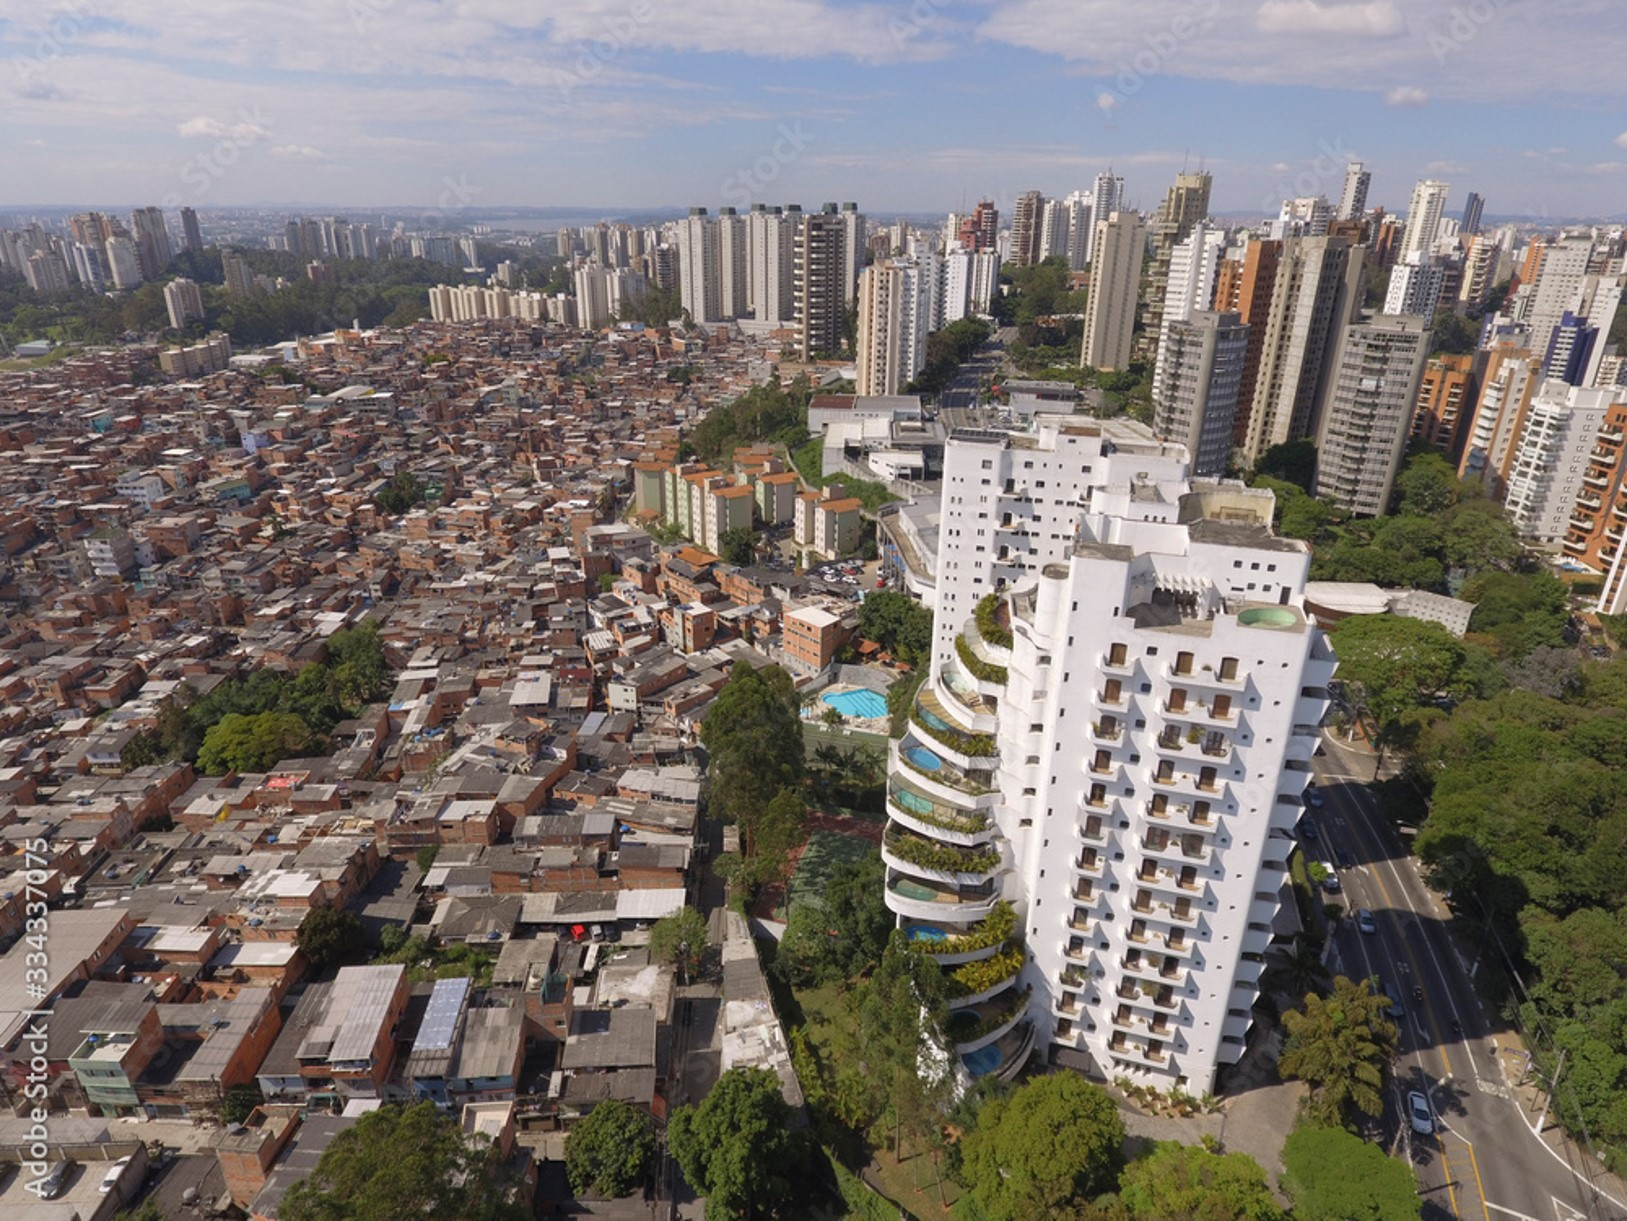
\includegraphics[height=0.2\textheight]{brazylia.jpg} % Skalowanie wg wysokości
    \end{figure}
\end{frame}

\begin{frame}{Turystyka i jej wpływ na lokalnych mieszkańców}
    Globalizacja silnie napędza też turystykę. Z jednej strony jako ludzie mamy możliwość zobaczyć
    miejsca na świecie, do których nasi przodkowie nie mieli nigdy dostępu. Z drugiej strony tu-
    rystyka ma w dużym stopniu negatywny wpływ na jakość życia rodowitych mieszkańców miejsc,
    które odwiedzamy. Nie musimy szukać daleko, żeby takie miejsce znaleźć, bo wystarczy zajrzeć
    do Florencji – stolicy włoskiej Toskanii. Rodziny mieszkające we florentyńskich kamienicach tracą
    wszystkich swoich sąsiadów, na rzecz krótkoterminowych najemców. Te mieszkania przeznaczone
    na krótkoterminowy najem nie należą też do właścicieli prywatnych, a do dużych korporacji, ukry-
    tych za kilkoma firmami „słupami”. Często w takich budynkach rachunki są liczone na ilość osób
    zameldowanych w takim budynku. Nikt nie liczy przejeżdżających tylko turystów, więc najwięcej
    płaci ta jedna rodzina, która nadal tam mieszka, co tylko potęguje problem
\end{frame}

\begin{frame}{Zagrożenia płynące z rozwoju globalizacji}
    Globalizacja niesie ze sobą ryzyko pogłębienia nierówności, w których bogate kraje bogacą się
    kosztem wyzysku biedniejszych regionów. Proces ten zagraża unikalnym tradycjom, wypieranym
    przez ujednoliconą, zachodnią popkulturę, oraz prowadzi do degradacji środowiska przez ma-
    sową produkcję i transport. Dodatkowo potężne korporacje zyskują wpływ dominujący nad suw-
    erennością państw, a ścisłe powiązania gospodarcze sprawiają, że lokalne kryzysy błyskawicznie
    rozprzestrzeniają się na cały świat.
\end{frame}

\begin{frame}{Bilans zysków i strat - podsumowanie}
    Bilans globalizacji to walka między ogromnymi możliwościami a nowymi zagrożeniami. Zysku-
    jemy przede wszystkim szybki wzrost gospodarczy, postęp technologiczny i łatwiejszy dostęp do
    wiedzy oraz tańszych produktów z całego świata. Straty to przede wszystkim pogłębiające się
    nierówności społeczne, wyzysk biedniejszych regionów oraz ogromne obciążenie dla środowiska i
    zanik lokalnych tradycji. Ostatecznie globalizacja jest procesem nieuchronnym, który jednym daje
    narzędzia rozwoju, a innych stawia przed ryzykiem marginalizacji.
\end{frame}

\nocite{*}
\begin{frame}[allowframebreaks]{Bibliografia}
    \printbibliography
\end{frame}

\begin{frame}{Zakończenie}
    Dziękuję za uwagę!
\end{frame}


\end{document}